\section{Control-Theoretic Training}

\begin{frame}
    \begin{center}
        \huge 3: \textbf{Unified Control-Theoretic Training}
    \end{center}
\end{frame}

\begin{frame}{Unified Control-Theoretic Training: Parametrization and Datasets}
    \footnotesize
    \visible<1->{
    Define the \textbf{configuration} of the observable system responses,}
    \begin{columns}
        \begin{column}{0.5\textwidth}
            \visible<2->{
            \vspace*{-0.1in}
            \begin{graybox}{Parameters}
                \visible<3->{
                \begin{figure}
                    \centering
                    \includegraphics[width=0.7\textwidth]{../../Chapter-3/Figures/parametrization.png}
                \end{figure}}
                \vspace*{-0.1in}
                \visible<4->{
                \begin{equation*}
                    \cP = \left\{\vp^{(l)} = \left(\vtheta^{(l)},\vxi^{(l)},\vu^{(l)}(t)\right)^\top\right\}_{l=1}^{N},\: t\in\cT
                \end{equation*}}
                \vspace*{-0.1in}
                \begin{itemize}
                    \item<5-> $\vtheta$: deployment and terminal conditions,
                    \item<6-> $\vxi$: materials properties, geometry, 
                    \item<7-> $\vu$: heat flux, pressure loads, etc.
                \end{itemize}
            \end{graybox}}
        \end{column}
        \begin{column}{0.5\textwidth}
            \visible<8->{
            \begin{graybox}{Dataset}
                \vspace*{-0.05in}
                \visible<9->{
                \begin{figure}
                    \centering
                    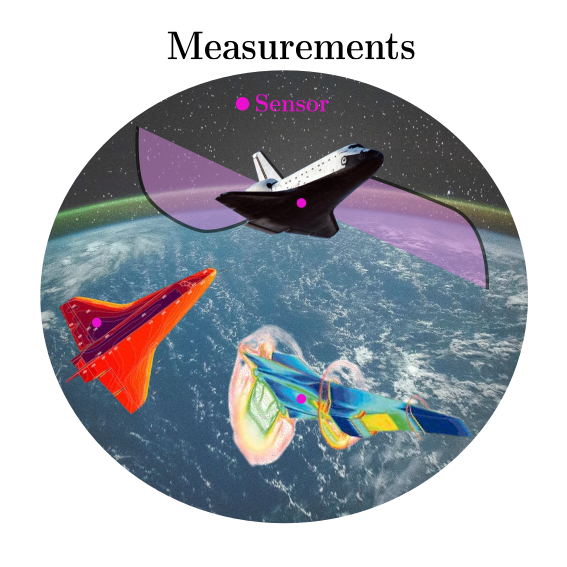
\includegraphics[width=0.5\textwidth]{../figs/pirom/sensors.png}
                \end{figure}}
                \vspace*{-0.2in}
                \visible<10->{
                \begin{equation*}
                    \cD = \left\{\vz_{\text{HF}}^{(l)}(t_k),\vu^{(l)}(t_k);\vp^{(l)}(t_k)\right\}_{l=1}^{N},\: t_k\in\cT'
                \end{equation*}}
                \vspace*{-0.1in}
                \begin{itemize}
                    \item<11-> $\vz_{\text{HF}}$: observable signals,
                    \item<12-> $\cT'=\left\{t_0,\dots,t_p\right\}$: time instances
                    \item<13-> $N$: number of trajectories (\textcolor{red}{$N \lessapprox 10$}).
                \end{itemize}
            \end{graybox}}
        \end{column}
    \end{columns}
\end{frame}

\begin{frame}{Unified Control-Theoretic Training: Problem Statement}
    \footnotesize
    \visible<1->{The \textbf{training problem} is defined as the \textbf{optimal control problem} (OCP),}
    \begin{columns}
        \begin{column}{0.35\textwidth}
            \visible<2->{
            \begin{graybox}{The Training Problem}
                \begin{align*}
                    \visible<3->{
                    \min_{\redvomega} & \:\cJ(\redvomega;\cD)}\\
                    \visible<6->{
                    \text{s.t.}\quad & \dot{\vy}^{(l)} = \vcQ\left(\vy^{(l)},\vp^{(l)};\redvomega\right)}\\
                    \visible<7->{
                    \vzero &= \vPsi_0\left(\vy^{(l)}(t_0),t_0;\vp^{(l)}\right)}\\
                    \visible<8->{
                    \vzero &= \vPsi_f\left(\vy^{(l)}(t_f),t_f;\vp^{(l)}\right)}
                \end{align*}        
            \end{graybox}}
        \end{column}
        \begin{column}{0.65\textwidth}
            \visible<2->{
            \begin{graybox}{Problem Components}
                \begin{itemize}
                    \item <3-> $\redvomega$: design parameters,
                    \item <3-> $\cJ$: loss functional,
                    \visible<4->{
                    \begin{equation*}
                        \cJ(\redvomega;\cD) = \frac{1}{N}\sum_{l=1}^{N}\left\{\varphi\left(\vy^{(l)}(t_f),t_f\right) + \int_{t_0}^{t_f}\ell\left(\vy^{(l)},\vz^{(l)}_{\text{HF}},\redvomega\right)dt\right\}
                    \end{equation*}}
                    \visible<5->{
                    \begin{equation*}
                        \varphi: \text{terminal loss},\: \ell: \text{running \textcolor{red}{observable} loss}
                        \vspace*{-0.15in}
                    \end{equation*}}
                    \item <6-> $\vcQ$: non-linear dynamics parametrized by $\redvomega$,
                    \item <6-> $\vy^{(l)}$: dynamical state for the $l$-th case,
                    \item <8-> $\vPsi_0$, $\vPsi_f$: initial and terminal constraints,
                \end{itemize}
            \end{graybox}}
        \end{column}
    \end{columns}
\end{frame}

\begin{frame}{Unified Control-Theoretic Training: Examples}
    \footnotesize
    \visible<1->{\textbf{Unified Control-theoretic} view for \textbf{reduced-order modeling} and \textbf{optimal control},}
    \begin{center}
        \visible<2->{$\textcolor{red}{\vomega(t)}=\redvTheta$: \textbf{parameters} (feedback controller),} \quad \visible<9->{$\textcolor{red}{\vomega(t)}=\textcolor{red}{\vbeta(t)}$: \textbf{hidden state} (no feedback controller)}
    \end{center}
    \vspace*{-0.1in}
    \begin{columns}
        \begin{column}{0.4\textwidth}
            \visible<3->{
            \begin{graybox}{Reduced-Order Modeling}
                \begin{align*}
                    \visible<4->{
                    \min_{\redvTheta} & \:\cJ(\redvTheta;\cD)}\\
                    \visible<5->{
                    \text{s.t.}\quad & \dot{\vy}^{(l)} = \vcQ\left(\vy^{(l)},\vp^{(l)};\redvTheta\right)}\\
                    \visible<6->{
                    \vzero &= \vPsi_0\left(\vy^{(l)}(t_0),t_0;\vp^{(l)},\redvTheta\right)}\\
                    \visible<7->{
                    \vzero &= \vPsi_f\left(\vy^{(l)}(t_f),t_f;\vp^{(l)},\redvTheta\right)}
                \end{align*}
            \end{graybox}}
            \visible<8->{
            Solve by, e.g.,
            \begin{itemize}
                \item Direct optimal control \textcolor{red}{(NODE)}
            \end{itemize}}
        \end{column}
        \begin{column}{0.6\textwidth}
            \visible<9->{
            \begin{graybox}{Optimal Control}
                \visible<10->{
                Let $\redvB = [\redvbeta^{(1)},\dots,\redvbeta^{(N)}]$, $\vY = \left[\vy^{(1)},\dots,\vy^{(N)}\right]$, and so on,}
                \begin{align*}
                    \visible<11->{
                    \min_{\redvB(t)} & \:\cJ(\redvB;\cD)}\\
                    \visible<12->{
                    \text{s.t.}\quad & \dot{\vY} = \bar{\vcQ}\left(\vY,\vP;\redvB\right)}\\
                    \visible<13->{
                    \vzero &= \bar{\vPsi}_0\left(\vY(t_0),t_0;\vP\right)}\\
                    \visible<14->{
                    \vzero &= \bar{\vPsi}_f\left(\vY(t_f),t_f;\vP\right)}
                \end{align*}
            \end{graybox}}
            \visible<15->{
            Solve by, e.g.,
            \begin{itemize}
                \item Indirect optimal control (\textcolor{red}{PMP}), but very \textbf{costly to solve}
            \end{itemize}}
        \end{column}
    \end{columns}
\end{frame}

\begin{frame}{Unified Control-Theoretic Training: Examples}
    \footnotesize
    \vspace*{0.05in}
    \visible<1->{\textbf{Direct one-step approach} (NODE-like training) sets $\textcolor{red}{\vomega(t)} = \textcolor{red}{\vTheta^{(j)}}$ and does the following,}
    \only<1>{
        \begin{figure}
            \centering
            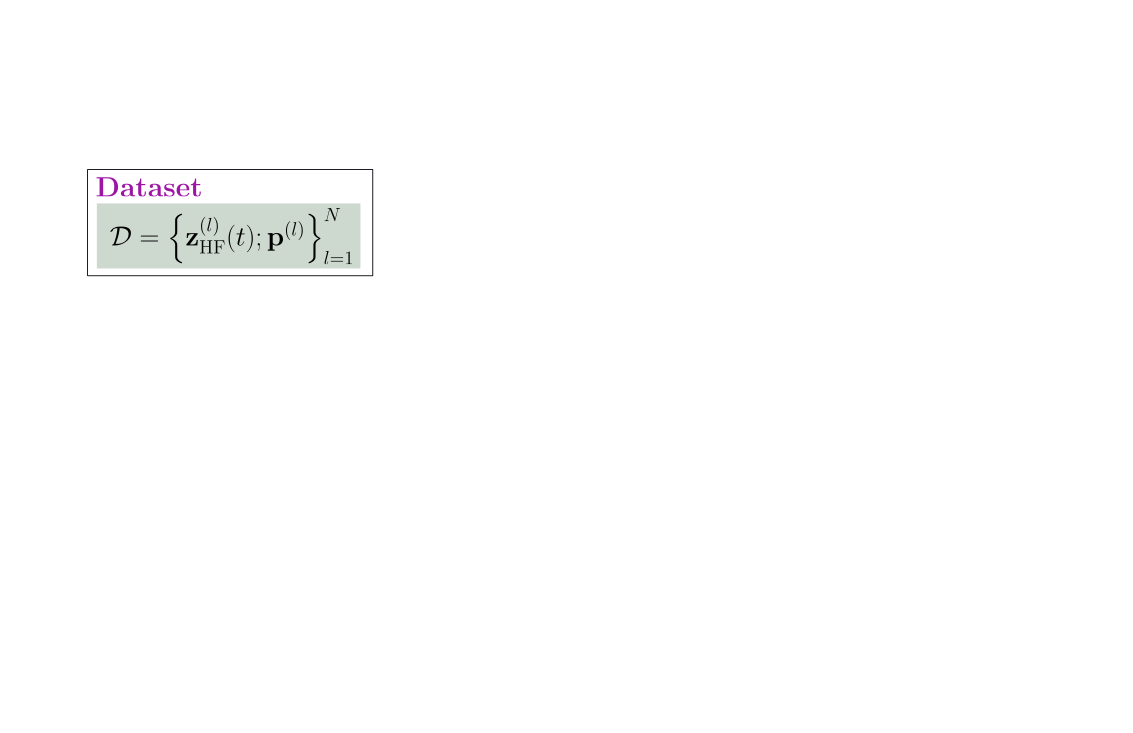
\includegraphics[width=0.8\textwidth]{../figs/pirom/one_step_1.png}
        \end{figure}}
    \only<2>{
        \begin{figure}
            \centering
            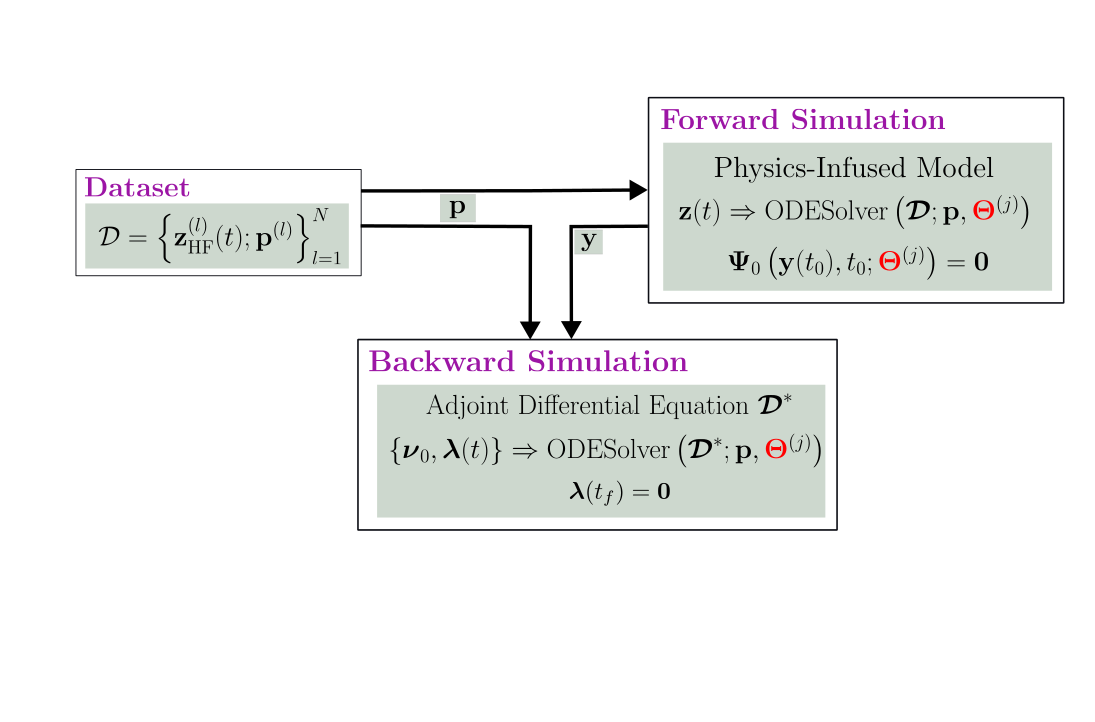
\includegraphics[width=0.8\textwidth]{../figs/pirom/one_step_2.png}
        \end{figure}}
    \only<3>{
        \begin{figure}
            \centering
            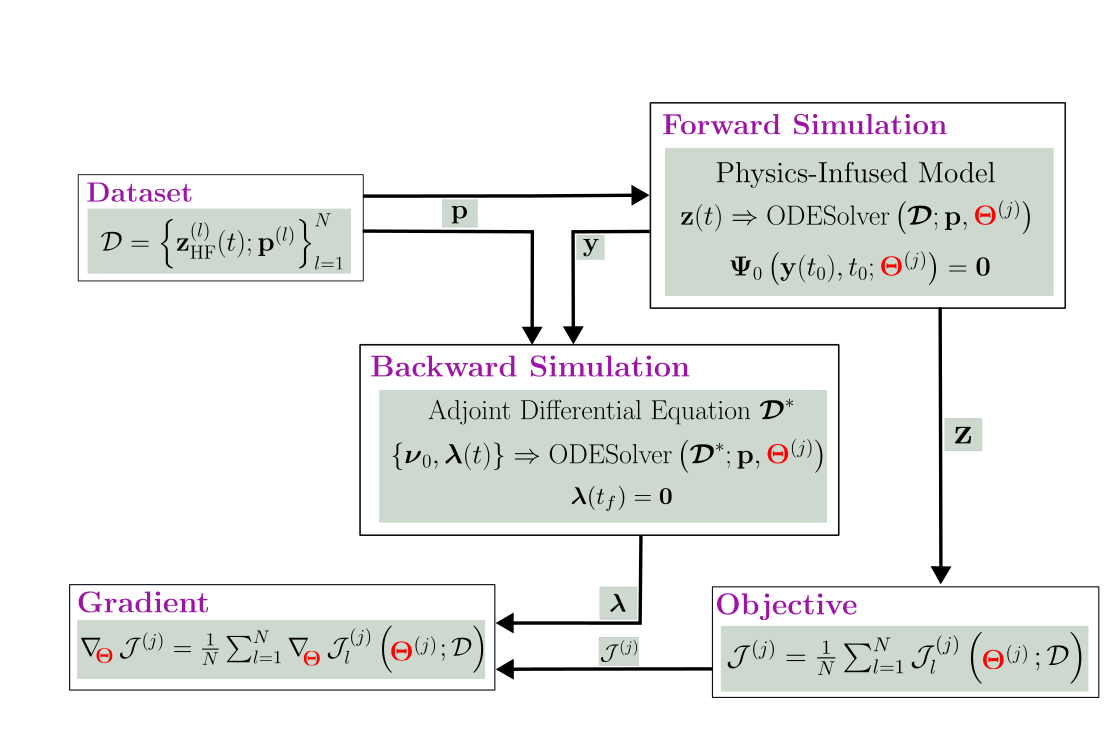
\includegraphics[width=0.8\textwidth]{../figs/pirom/one_step_3.png}
        \end{figure}}
    \only<4>{
        \begin{figure}
            \centering
            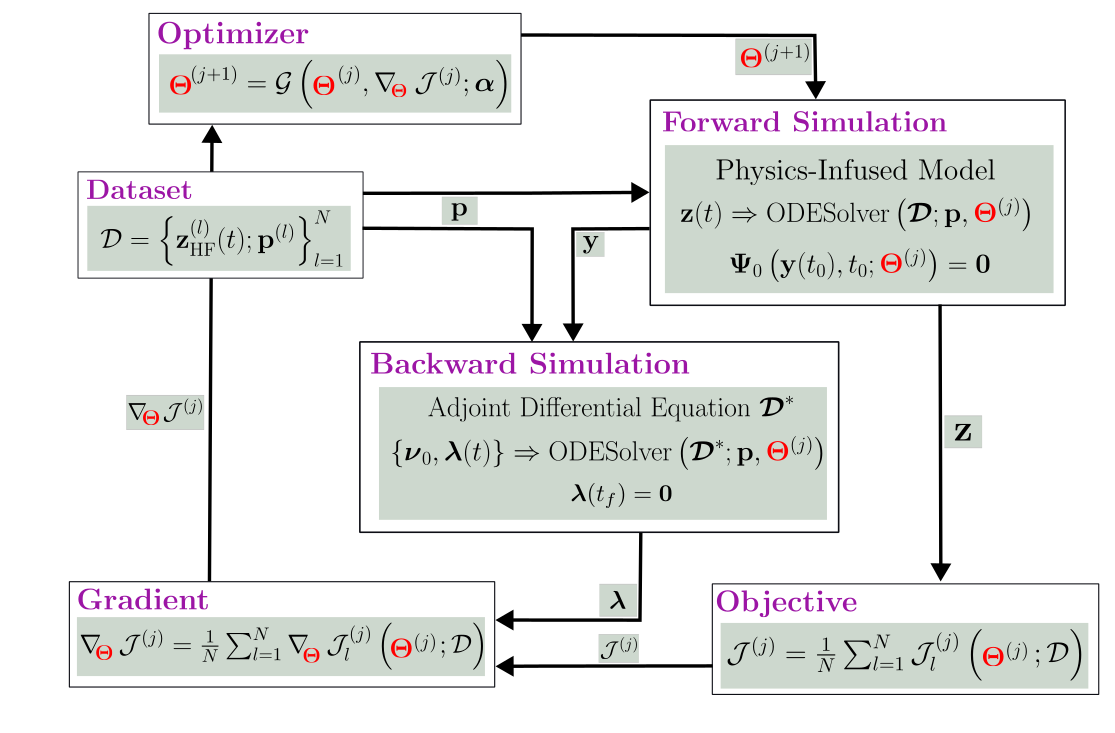
\includegraphics[width=0.8\textwidth]{../figs/pirom/one_step_4.png}
        \end{figure}}
    \only<5>{
        \begin{figure}
            \centering
            \includegraphics[width=0.7\textwidth]{../figs/pirom/one_step_5.png}
        \end{figure}}
\end{frame}

\begin{frame}{Unified Control-Theoretic Training: Examples}
    \footnotesize
    \vspace*{0.05in}
    \visible<1->{\textbf{Indirect two-step approach} sets $\textcolor{red}{\vomega^{(l)}(t)} = \textcolor{red}{\vbeta^{(l)}(t)}$ for $l=1,\dots,N$ and does the following,}
    \vspace*{-0.1in}
    \only<2>{
        \begin{figure}
            \centering
            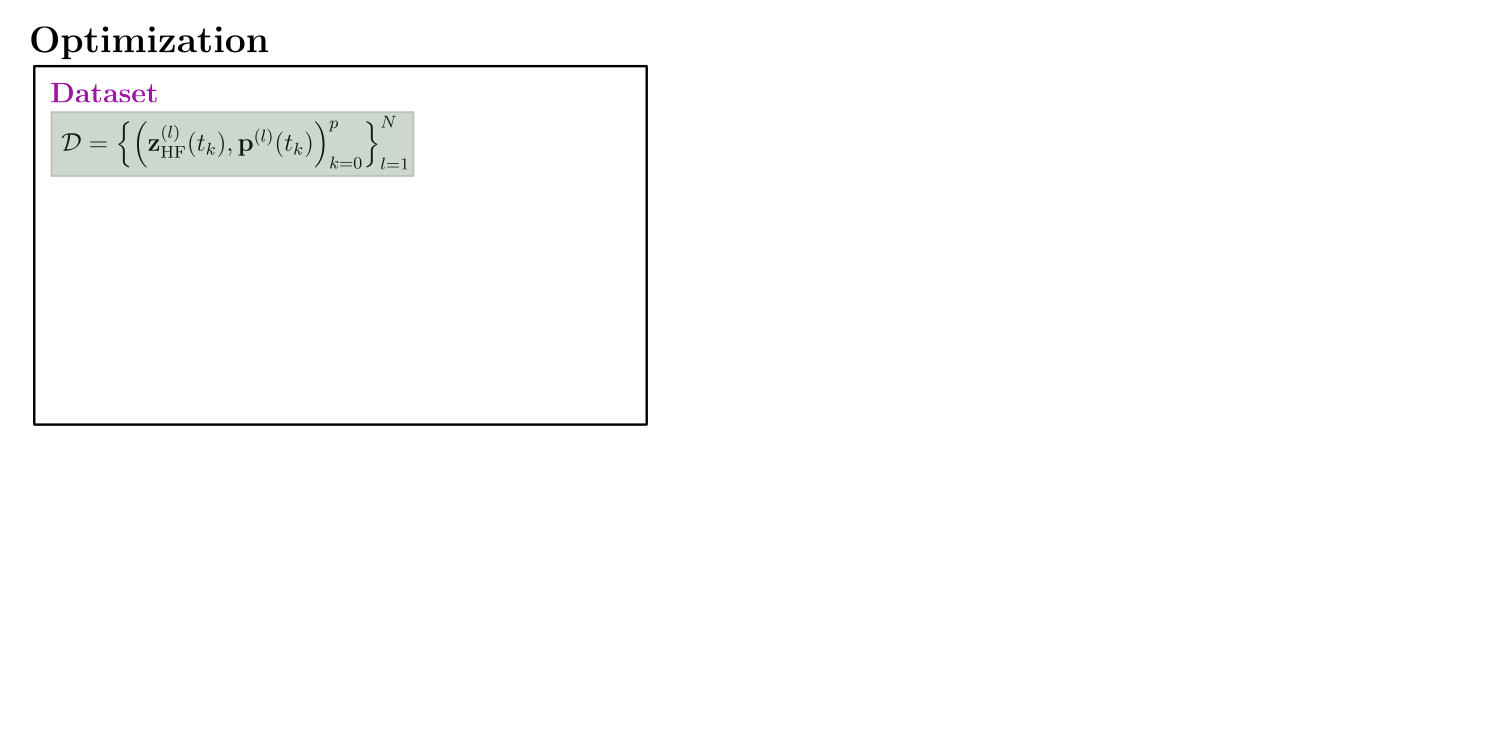
\includegraphics[width=0.8\textwidth]{../figs/pirom/two_step_1.png}
        \end{figure}}
    \only<3>{
        \begin{figure}
            \centering
            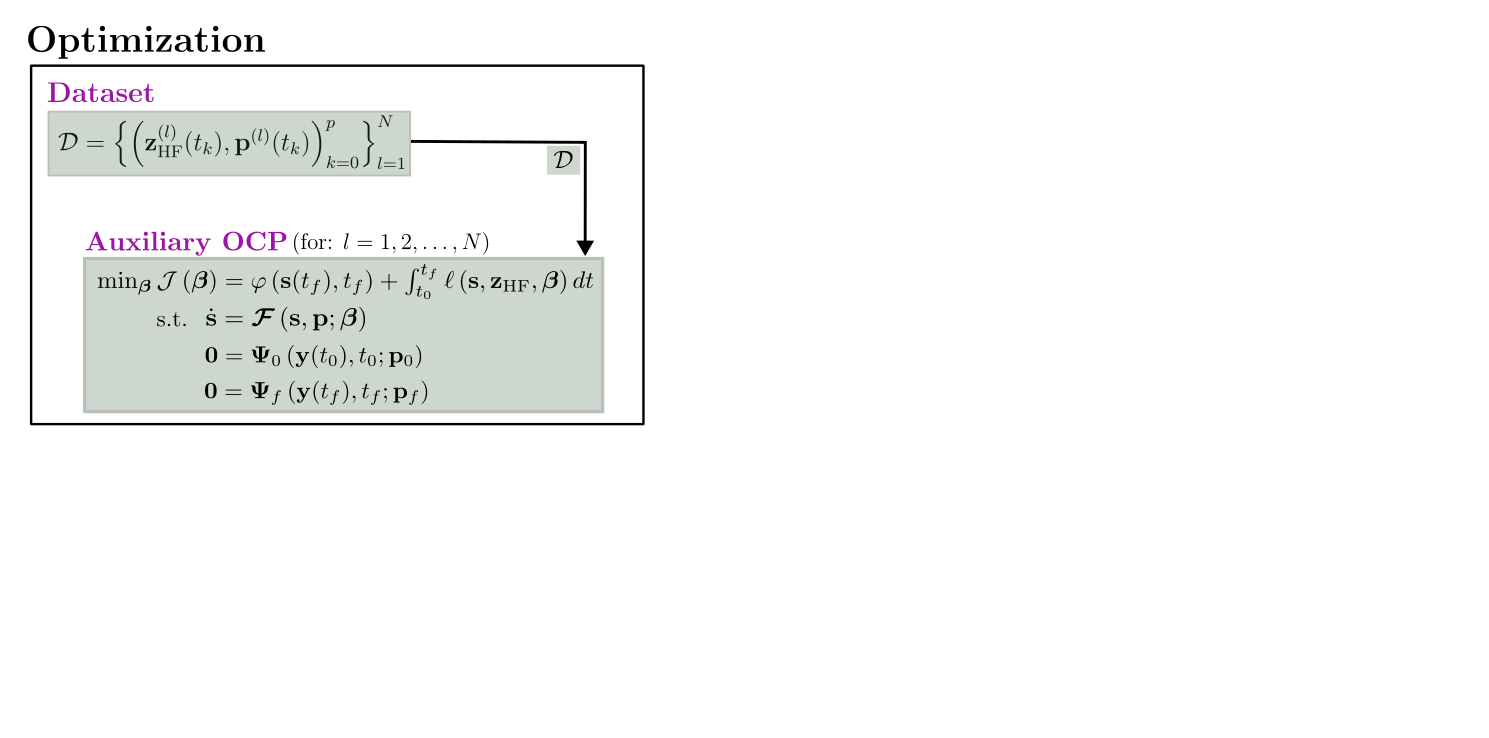
\includegraphics[width=0.8\textwidth]{../figs/pirom/two_step_2.png}
        \end{figure}}
    \only<4>{
        \begin{figure}
            \centering
            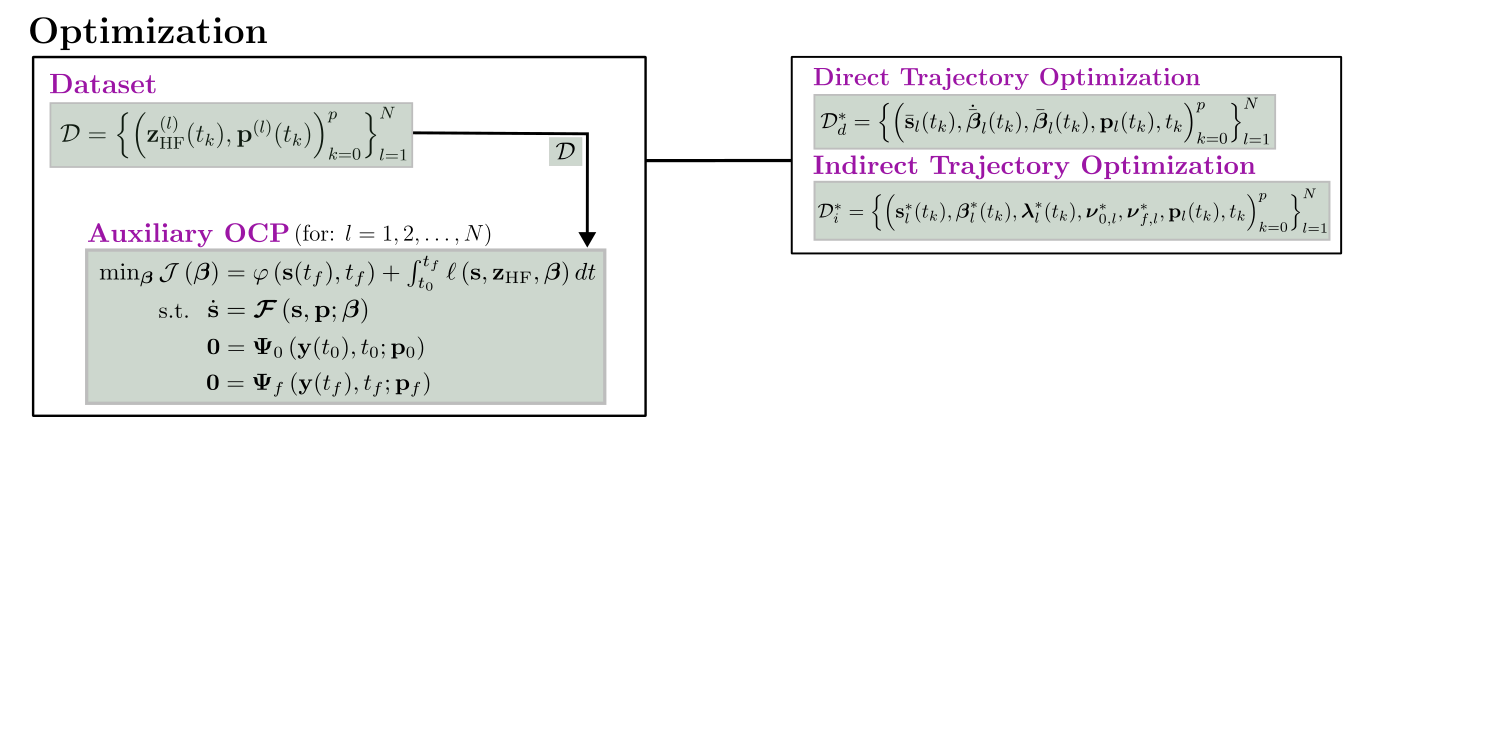
\includegraphics[width=0.8\textwidth]{../figs/pirom/two_step_3.png}
        \end{figure}}
    \only<5>{
        \begin{figure}
            \centering
            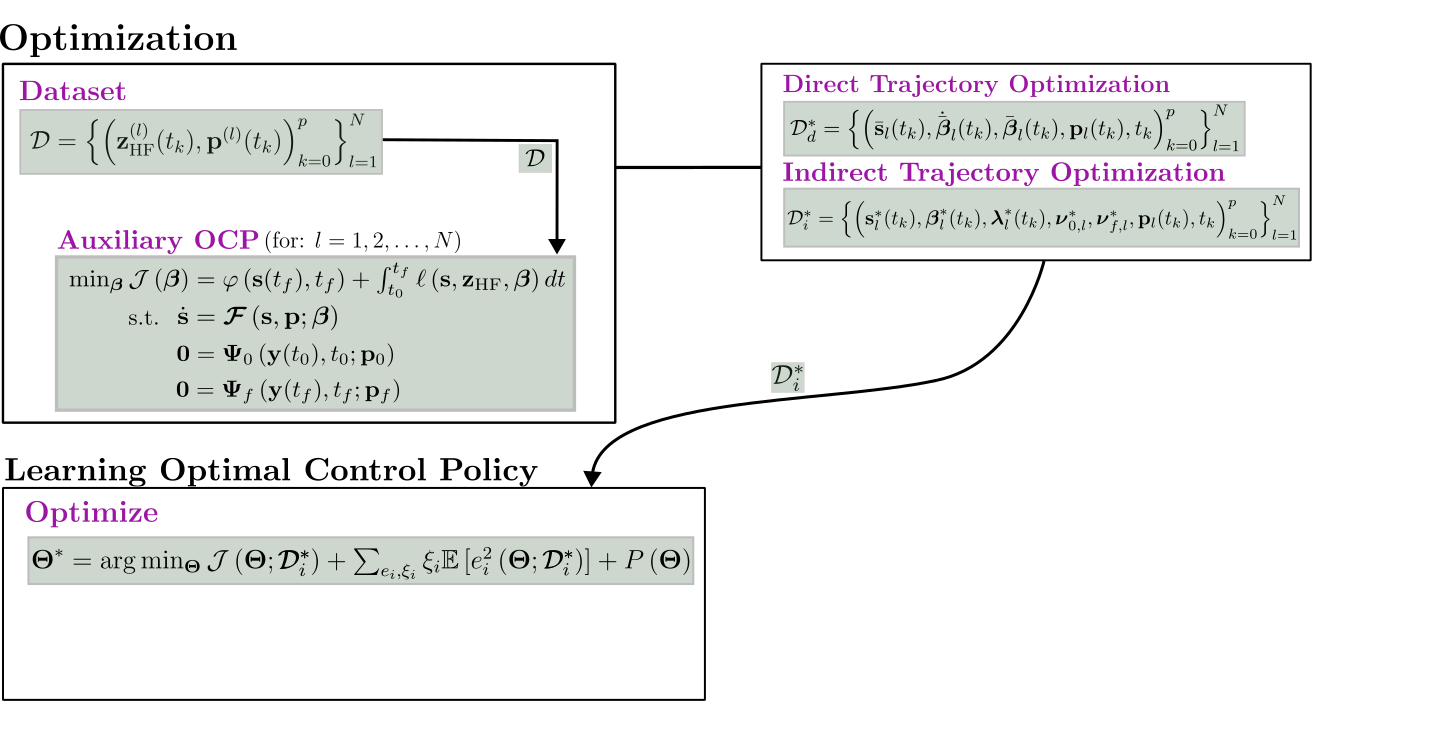
\includegraphics[width=0.8\textwidth]{../figs/pirom/two_step_4.png}
        \end{figure}}
    \only<6>{
        \begin{figure}
            \centering
            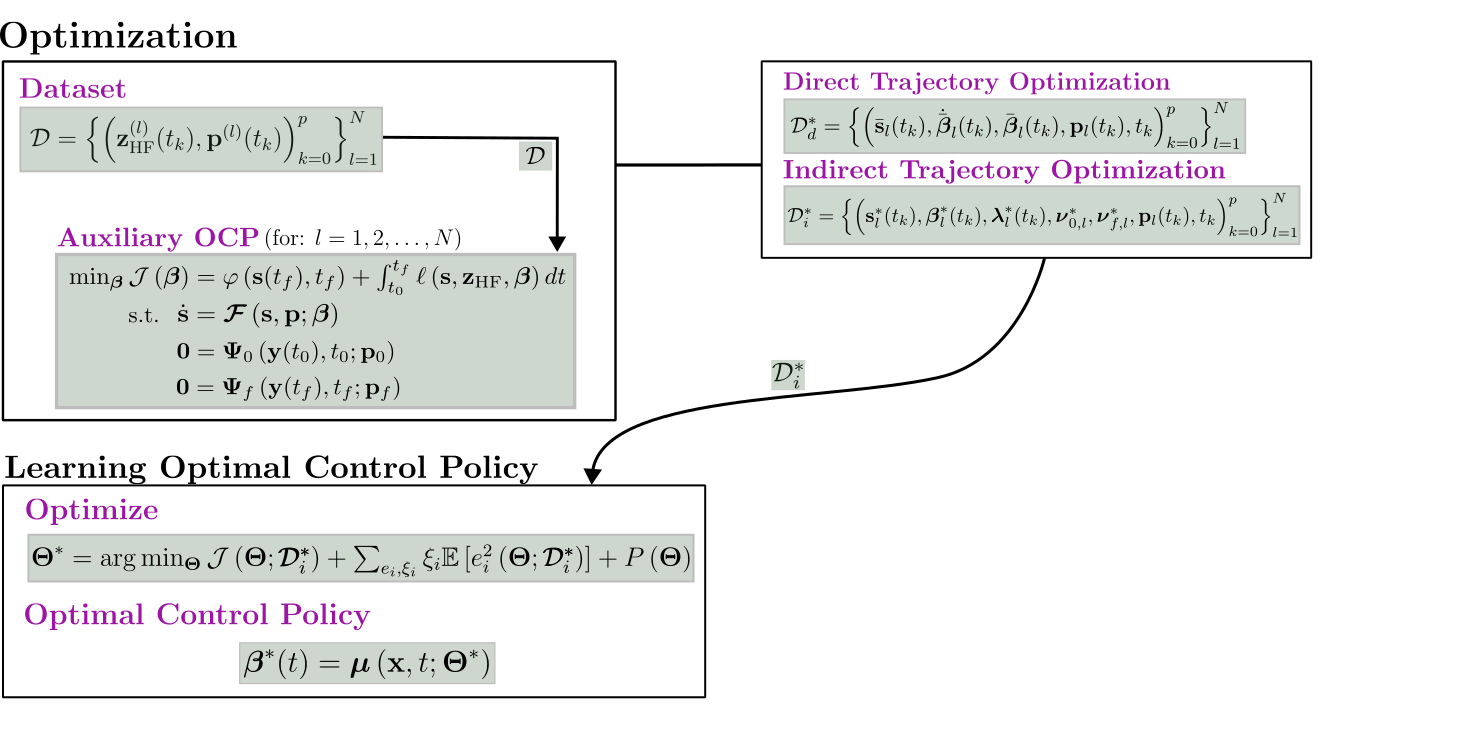
\includegraphics[width=0.8\textwidth]{../figs/pirom/two_step_5.png}
        \end{figure}}
    \only<7>{
        \begin{figure}
            \centering
            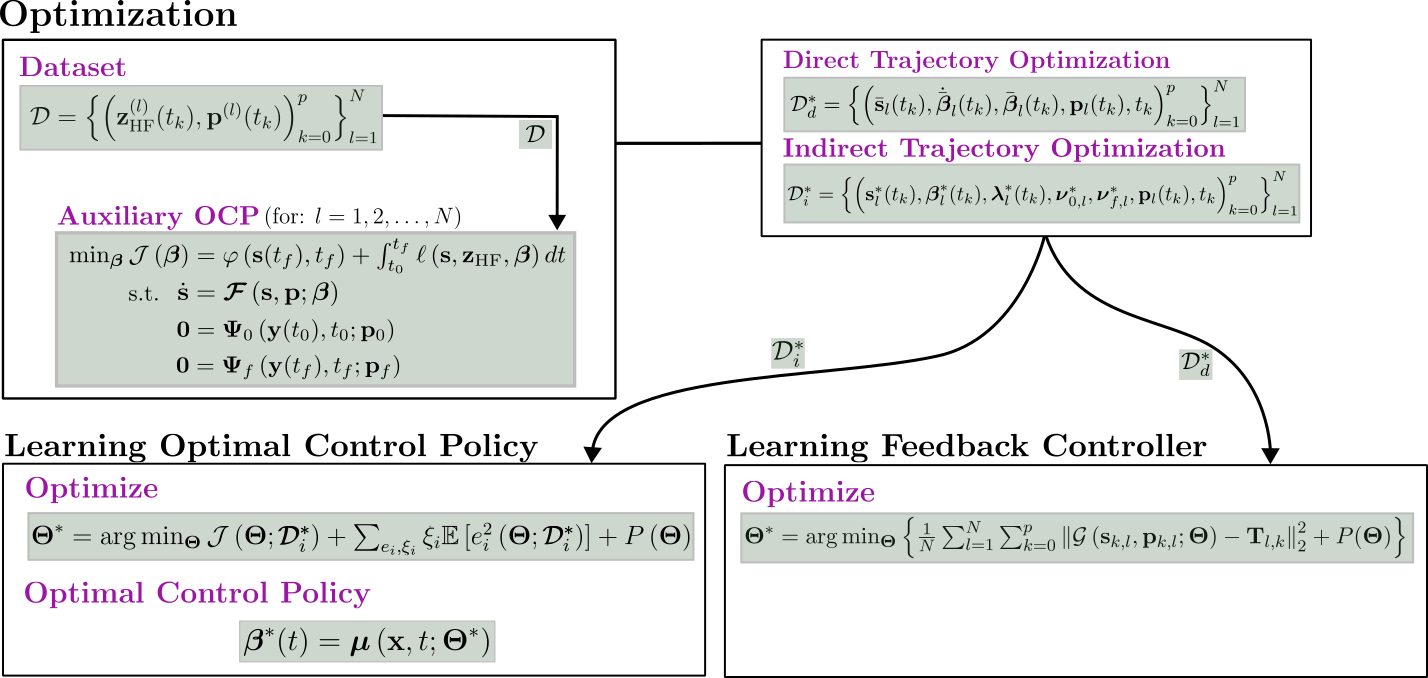
\includegraphics[width=0.8\textwidth]{../figs/pirom/two_step_6.png}
        \end{figure}}
    \only<8>{
        \begin{figure}
            \centering
            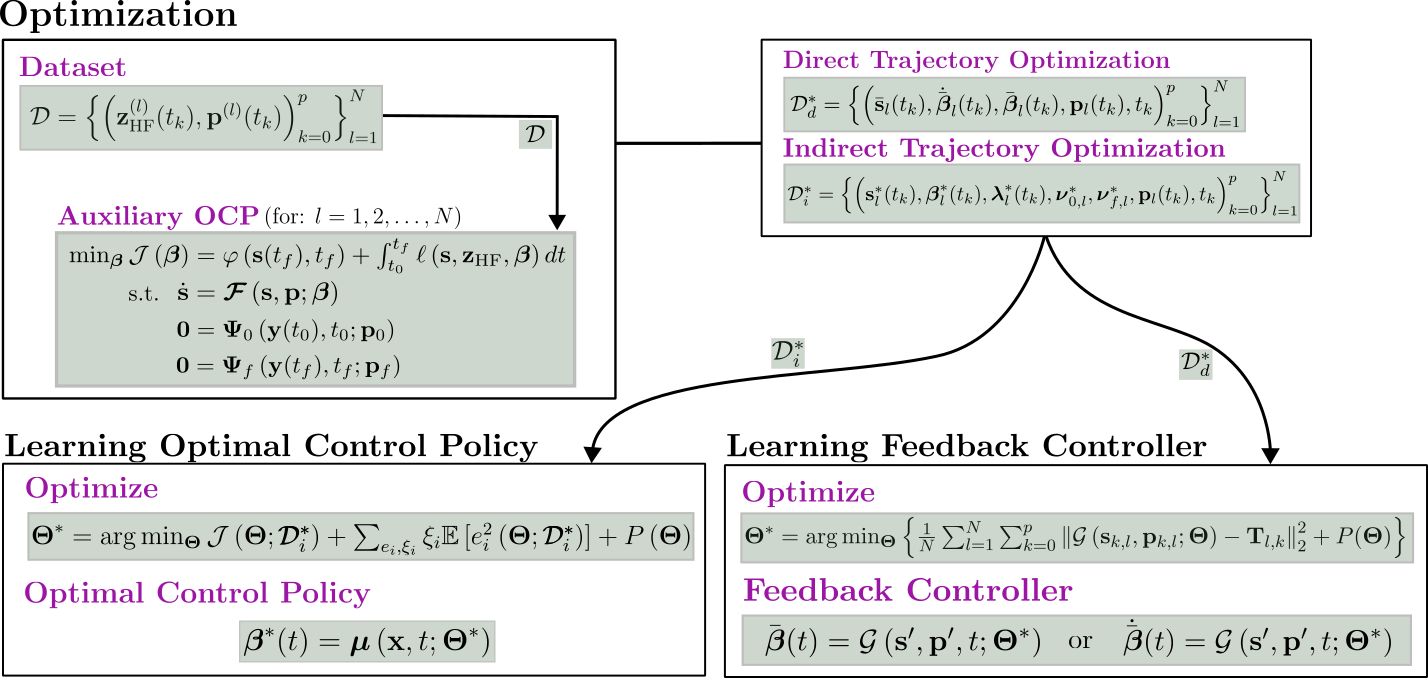
\includegraphics[width=0.8\textwidth]{../figs/pirom/two_step_7.png}
        \end{figure}}
    \visible<2->{
    \begin{center}
        \vspace*{-0.1in}
        {\tiny
        $\vs$: physics state, $\vcF$: physics-infused model, $\vbeta$: hidden state, $\vlambda$: costate, $\vnu_0$, $\vnu_f$: boundary sensitivities, $\vmu$: optimal control policy, $\vp$: parameters, $\mathbf{T}_{l,k}$: desired target, $P(\vTheta)$: regularization term}
    \end{center}}
\end{frame}

\begin{frame}{Unified Control-Theoretic Training: Optimal Control Policy}
    \footnotesize
    \visible<1->{Consider the following extension with \textbf{dynamic programming} theory,}
    \begin{columns}
        \begin{column}{0.35\textwidth}
            \centering
            \visible<2->{
            \begin{graybox}{Field of Extremals}
                \centering
                \visible<3->{
                Indirect solutions: $\cD_i$
                \begin{figure}
                    \centering
                    \includegraphics[width=0.9\textwidth]{../../Chapter-3/Figures/tube.png}
                \end{figure}}
                \visible<4->{
                \textbf{TPBVP solutions are HJB characteristics!}}
            \end{graybox}}
        \end{column}
        \begin{column}{0.65\textwidth}
            \centering
            \visible<5->{
            \begin{graybox}{Dynamic Programming}
                \visible<6->{
                Value function,
                \vspace*{-0.1in}
                \begin{equation*}
                    \cV(\vx,t) = \min_{\vbeta}\left\{\varphi\left(\vs(t_f),t_f\right) + \int_{t_0}^{t_f}\ell\left(\vs,\vz_{\text{HF}},\vbeta\right)dt\right\}
                \end{equation*}}
                \visible<7->{
                HJB PDE (\textbf{costly to solve} due to curse of dimensionality),
                \begin{equation*}
                    -\frac{\partial \cV}{\partial t} = \min_{\vbeta}\left\{\ell\left(\vs,\vz_{\text{HF}},\vbeta\right) + \frac{\partial \cV}{\partial \vs}^\top \vcF\left(\vs,\vp,\vbeta\right)\right\}
                \end{equation*}}
                \visible<8->{
                Pontryagin's Minimum Principle (PMP),
                \begin{equation*}
                    \vbeta^*(t) = \vmu^*(\vx,t) = \arg\min_{\vbeta}\left\{\ell\left(\vs,\vz_{\text{HF}},\vbeta\right) + \vlambda^\top \vcF\left(\vs,\vp,\vbeta\right)\right\}
                \end{equation*}}
            \end{graybox}}
        \end{column}
    \end{columns}
    \begin{center}
        {\tiny HJB: Hamilton-Jacobi-Bellman, $\vs$: physics state, $\vcF$: physics-infused model, $\vbeta$: hidden state, $\vlambda$: costate, $\vmu^*$: optimal control policy, $\vp$: parameters}
    \end{center}
\end{frame}

\begin{frame}{Unified Control-Theoretic Training: Optimal Control Policy}
    \footnotesize
    \visible<1->{We \textbf{can learn the value function} using supervised \textbf{physics-informed} learning,}
    \begin{columns}
        \begin{column}{0.55\textwidth}
            \visible<2->{
            \begin{graybox}{Function Approximation}
                \visible<3->{
                \begin{equation*}
                    \tilde{\cV}(\vx,t) = \sum_{i=1}^{m} \redTheta_i(t)\phi_i(\vx) = \redvTheta(t)^\top \vPhi(\vx)
                \end{equation*}}
                \vspace*{-0.1in}
                \begin{itemize}
                    \item<4-> \textbf{Value Function}: $e_V(\redvTheta;\vx) = \redvTheta^\top\vPhi(\vx) - \cV^*$
                    \item<5-> \textbf{HJB}: $e_{\text{HJB}}(\redvTheta;\vx) = \left(\frac{\Delta\redvTheta}{\Delta t}\right)^\top\vPhi(\vx) + \cH^*$
                    \item<6-> \textbf{Hamiltonian}: $e_{\cH}(\redvTheta;\vx) = \ell^* + \redvTheta^\top\frac{\partial\vPhi}{\partial\vs}\vcF^* - \cH^*$
                    \item<7-> \textbf{PMP}: $e_{\text{PMP}}(\redvTheta;\vx,\vbeta) = \frac{\partial\ell^*}{\partial\vbeta} + \redvTheta^\top\frac{\partial\vPhi}{\partial\vs}\frac{\partial\vcF^*}{\partial\vbeta} - \cH_{\vbeta}^*$
                    \item<8-> \textbf{Costate}: $e_{\vlambda}(\redvTheta;\vx) = \redvTheta^\top\frac{\partial\vPhi}{\partial\vs} - \vlambda^*$
                \end{itemize}
            \end{graybox}}
        \end{column}
        \begin{column}{0.5\textwidth}
            \visible<9->{
            \begin{graybox}{Value Function Learning}
                \visible<10->{
                For $k=1,2,\dots,p$,
                \vspace*{-0.1in}
                \begin{equation*}
                    \min_{\redvTheta_k}\: \cG(\redvTheta_k;\cD_i) + \eta\left\|\vLambda\redvTheta_k\right\|_1  
                \end{equation*}}
                \visible<11->{
                Physics-informed loss,
                \vspace*{-0.1in}
                \begin{equation*}
                    \cG(\redvTheta_k;\cD_i) = \sum_{e_i\in\cR,\xi_i\in\Xi}\xi_i \mathbb{E}\left[e_i^2\left(\redvTheta_k;\vx\right)\right]
                \end{equation*}}
                \visible<12->{
                \vspace*{-0.1in}
                where,}
                \vspace*{-0.05in}
                \begin{align*}
                    \visible<13->{
                    \cR &= \left\{e_V,e_{\text{HJB}},e_{\cH},e_{\text{PMP}},e_{\vlambda}\right\}}\\
                    \visible<14->{
                    \Xi &= \left\{\xi_V,\xi_{\text{HJB}},\xi_{\cH},\xi_{\text{PMP}},\xi_{\vlambda}\right\}}\\
                    \visible<15->{
                    \vLambda_{ii} &= \frac{1}{\left|\redvTheta^*_{k,i}\right| + \delta}}
                \end{align*}
            \end{graybox}}
        \end{column}
    \end{columns}
    \begin{center}
        {\tiny $\Box^*$: optimal quantity, $\Box_k$: quantity at discrete time $t_k$, $\cH$: Hamiltonian, $\vPhi$: basis functions, $\vTheta^*$: non-sparse parameters, $m$: number of basis functions, $\delta = \min\left(\left|\vTheta^*\right|\right)$}
    \end{center}
\end{frame}